\section{Results and Tests}
As described earlier, we decided to use a simlpe program that only copied the input registers into the output registers. This simplifies testing the power consumption exploring different techniques, like polling, interrupts and energy modes. 

	\subsection{Testing for correctness}
	\begin{figure}[h]
		\centerline{
			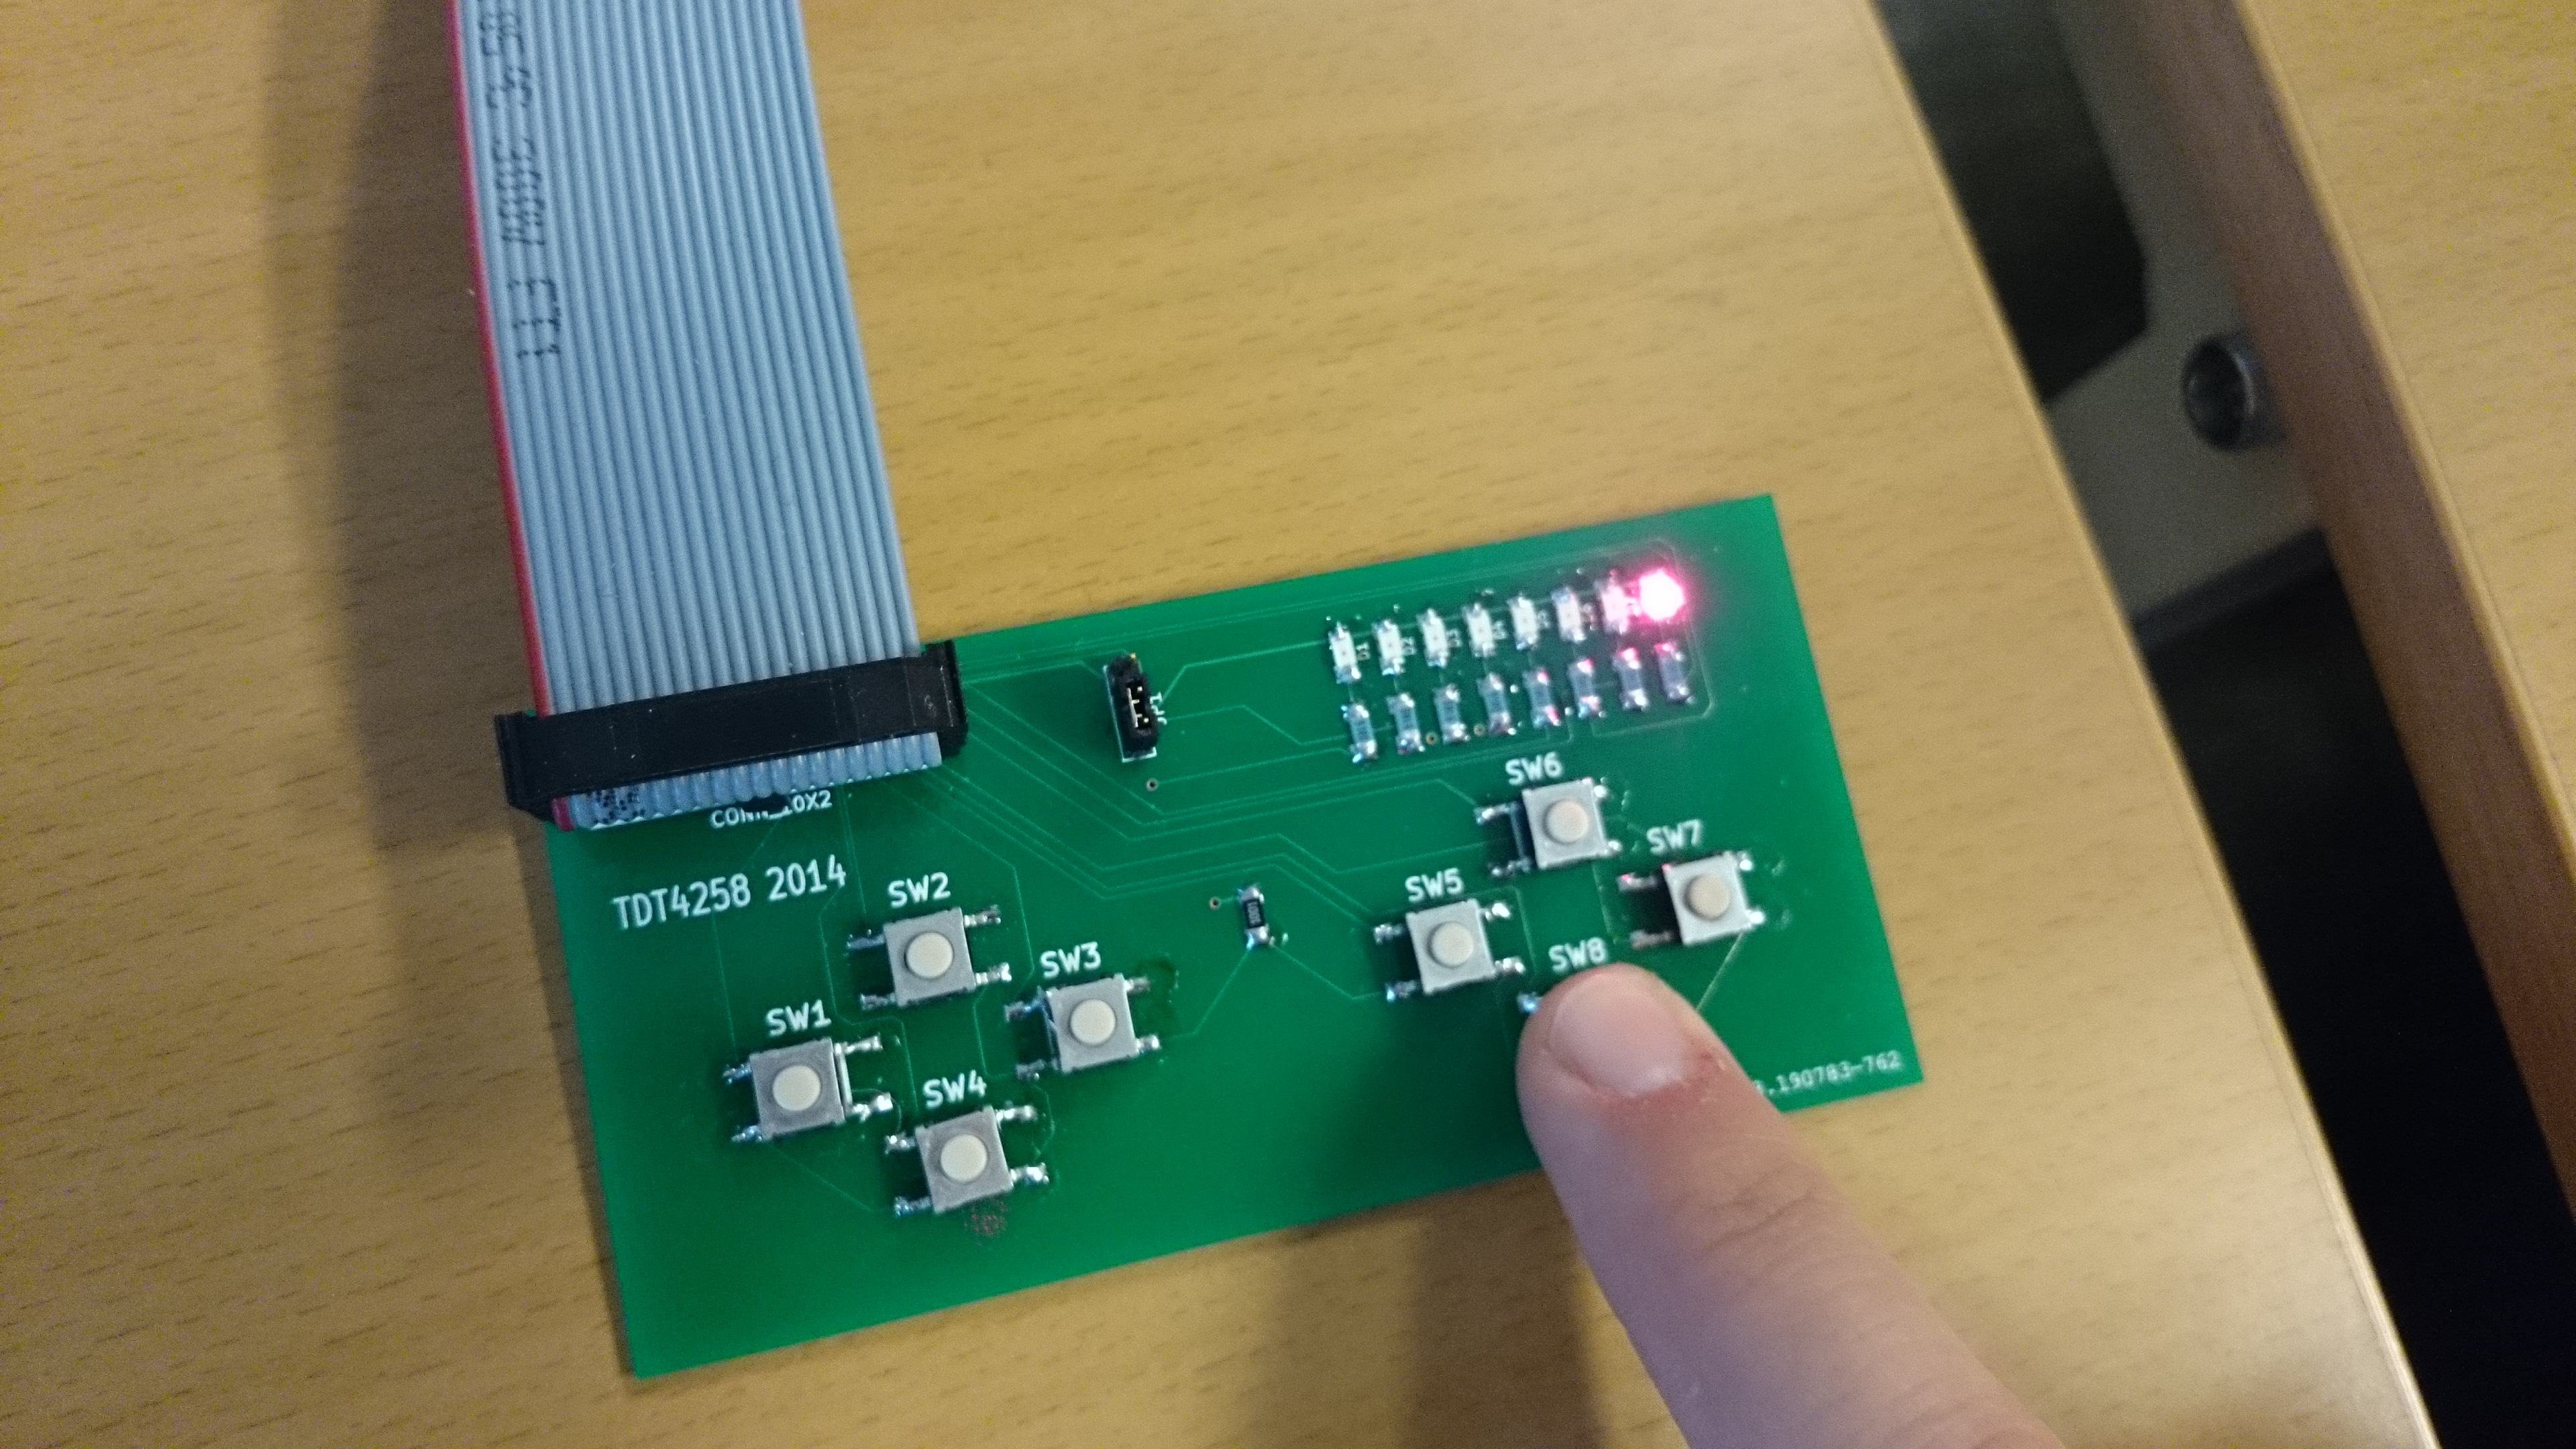
\includegraphics[width=0.5\textwidth]{img/test_correctness.jpg}
		}
		\caption{Verifying that the buttons and LEDs work correctly}
		\label{fig:test_correctness}
	\end{figure}
Testing the correctness for this simple proggram was easy. On every build, we confirmed that each button press lit the LED with the same number. Each LED should be on as long as the corresponding button is pressed. Se figure \ref{fig:test_correctness}.

	\subsection{Testing the energy effectiveness}
	In order to test the energy consumption of our system, we used the \emph{energyAware Profiler} provided by to us by Silicon Labs. We conducted the three following tests:

		\paragraph{Test 1 - No button press} 
		The system was run idle for ten seconds while the average amperage was measured. This test is important, because the system should consume less energy when it is in use.

		\paragraph{Test 2 - Button press}
		The system was run with buttons 1 and 8 held down continiously, which made LED 1 and 8 light during the whole test. The test was run for ten seconds, and average amperage was measured. We tested this, because we wanted to find out tetete

		\paragraph{Test 3 - Button press interval}



	\begin{itemize}
		\item
		\emph{Test 1 - No button press} \\
		The system was run idle for ten seconds. Average amperage was measured.

		\item
		\emph{Test 2 - Button press} \\
				
		\item
		\emph{Test 3 - Button press}
		The system was run for ten seconds, and button 1 was pressed down and released immediatly twice a second. Average amperage was measured.
	\end{itemize}

	These test were chosen to 
	We used a handheld stopwatch for all the tests. The sample trace was dumped into a raw text file for further processing in a spreadsheet.
